\chapter{Introduzione}
\label{chap:intro}

Questa tesi rappresenta la terza ed ultima parte dello stage++\footnote{Lo stage++ è un progetto unico, formato dall'unione di tre esami: project work, stage e tesi.},
realizzato in collaborazione con extrategy, il Prof. Francesco De Angelis e con il collega e amico Marco D'Argenio.
In questo stage ci è stato chiesto di realizzare un'applicazione per la domotica pensata per l'ufficio che prevedesse l'uso dei beacon, ovvero dei piccoli trasmettitori bluetooth che permettono la geolocalizzazione interna negli edifici. 
Proprio per questo motivo, il nome che abbiamo deciso di dare al nostro prodotto è: "Proximity System".

Gli obiettivi che dovevamo raggiungere con questo progetto erano numerosi, ragion per cui, io e Marco, ci siamo divisi il carico in maniera bilanciata e logica.
Io ho trattato tutti gli argomenti inerenti al backend e ai beacon. 
Marco, invece, ha trattato gli argomenti relativi al frontend dell'applicazione e ha studiato il BMC\footnote{Business Model Canvas} del prodotto per vedere la fattibilità dello stesso da un punto di vista economico. 
Questi argomenti non verranno trattati qui, ma nella tesi di Marco:"Analisi e sviluppo di un sistema software per la domotica d'ufficio: il frontend di Proximity System".

In sintesi, il progetto prevede tre parti: 
\begin{enumerate}
\item Il backend in esecuzione su Raspberry PI
\item Una web app per l'amministrazione del sistema
\item Un'app mobile per gestire i dispositivi
\end{enumerate}
Tutte e tre le componenti hanno una cosa in comune, sono tutte scritte in Javascript.

In questa tesi vedremo in dettaglio il primo punto e in generale come utilizzare lo stack MEAN\index{MEAN} per lo sviluppo di applicazioni web rispetto al tradizionale stack LAMP e come le WebSocket possano aumentare drasticamente le performance di un'applicazione real-time.

Il codice completo del progetto è disponibile nei due repository
\begin{enumerate}
\item \url{www.github.com/e-xtrategy/unicam-beacon-server}
\item \url{www.github.com/e-xtrategy/unicam-ionic-beacon-app}
\end{enumerate} 
Il primo contiene sia il backend con le API REST che la web app in Angular.
Il secondo contiene l'App Ionic compatibile con Android, iOS e, parzialmente (almeno per ora), Ubuntu Touch. 

\section{Analisi e progettazione}
La fase di analisi e di progettazione non si è sviluppata in maniera tradizionale, in quanto extrategy basa lo sviluppo di software sulle metodologie agili, più adatte ad ambienti dinamici come lo è il web.
Fra le pratiche promosse da questi metodi ci sono la formazione di team di sviluppo piccoli, cross-funzionali e auto-organizzati, 
lo sviluppo iterativo e incrementale, la pianificazione adattiva, e il coinvolgimento diretto e continuo del cliente nel processo di sviluppo.

Per essere precisi, abbiamo utilizzato un mix tra Scrum e Kanban.
Con Scrum\cite{scrum}\index{Scrum}, il prodotto viene realizzato tramite una serie di iterazioni a intervalli regolari chiamate sprint\index{Sprint} che danno al team un framework per consegnare al cliente del codice con una cadenza costante.
L'idea è quella che degli sprint frequenti rinforzano l'importanza di fare delle giuste stime e permettono di ricevere feedback in tempo reale sul lavoro svolto.
Ogni sprint è caratterizzato da questi quattro riti:
\begin{enumerate}
\item \textbf{Pianificazione}: un incontro iniziale in cui definire cosa fare con lo sprint corrente.
\item \textbf{Scrum giornaliero}: un mini incontro giornaliero della durata di una decina di minuti per sincronizzare il team. 
\item \textbf{Demo}: un incontro per illustrare il lavoro svolto dal team.
\item \textbf{Retrospettiva}: una revisione di ciò che si è stato fatto per farlo meglio la volta successiva.
\end{enumerate} 

Kanban\cite{kanban}\index{kanban} ci è d'aiuto durante gli sprint per tenere sott'occhio tramite una board l'avanzamento del nostro progetto.
Con questa metodologia il lavoro dell'intero team gira intorno alla kanban board, uno strumento utilizzato per visualizzare e ottimizzare il flusso del lavoro per tutto il team.
Mentre delle lavagne o intere pareti sono popolari per molti team, le board virtuali sono una caratteristica cruciale per lo sviluppo di software con le metodologie agile per la loro tranciabilità, facilità di collaborazione e accessibilità da diverse località.

Al di là che la board sia fisica o digitale, la sua funzione è quella di assicurare che il lavoro del team sia visualizzato, che il flusso sia standardizzato e che ogni imprevisto sia immediatamente visualizzato e risolto.
una kanban board di base ha tre step: To Do, In Progress e Done.
È ovvio che non c'è nessun vincolo sulla gestione del flusso e esso dipende da diversi fattori.
La metodologia kanban è basata sulla trasparenza del lavoro svolto e sulla comunicazione,
perciò  la kanban board dovrebbe essere vista come unica fonte di verità per il team. 

Questa impostazione crea l'esigenza di una piattaforma in grado di tenere traccia dello sviluppo del software e delle user-stories da implementare, capace anche di coordinare gli sviluppatori dedicati a quel caso.
Nonostante kanbanize probabilmente è una delle soluzione online più adatte ad implementare la metodologia Kanban, abbiamo scelto Trello perché il nostro piccolo team non necessita di applicare alla lettera Kanban con tutte le procedure consigliate per la gestione del flusso, e una semplice todo list era più che sufficiente.
 
Trello\index{Trello}\cite{trello} é un gestore di progetti basato sul web, originariamente realizzato da Fog Creek Soft-ware nel 2011.
In questo caso il progetto è rappresentato da schede, che contengono liste corrispondenti ad elenchi di attività. 
Le liste sono formate da card, che rappresentano le singole attività. 
Le card sono tenute a passare da una lista all'altra, tramite la funzione drag-and-drop; per via del generico flusso di una card, essa dovrebbe passare dalla lista delle cose da fare a quelle fatte, al momento del passaggio dall'idea alla realizzazione dell'attività in questione.
Nello specifico le card rappresentano le user-stories, funzionalità utile al raggiungimento di un obiettivo di business, una descrizione appositamente non dettagliata che il software deve avere e che alimenti la discussione tra il cliente/utente e lo sviluppatore.
Più programmatori possono essere assegnati alle card, ed insieme alle relative schede, possono essere raggruppati in organizzazioni differenti. 
Ogni card può accettare commenti, allegati, voti, date di scadenza e liste di controllo.
La suddivisione di un progetto in schede/liste, a loro volta suddivise in card formano una gerarchia di dati su misura che facilita la gestione efficace dei progetti stessi, nonché delle attività dell'intera organizzazione.
\begin{figure}[h]
\centering
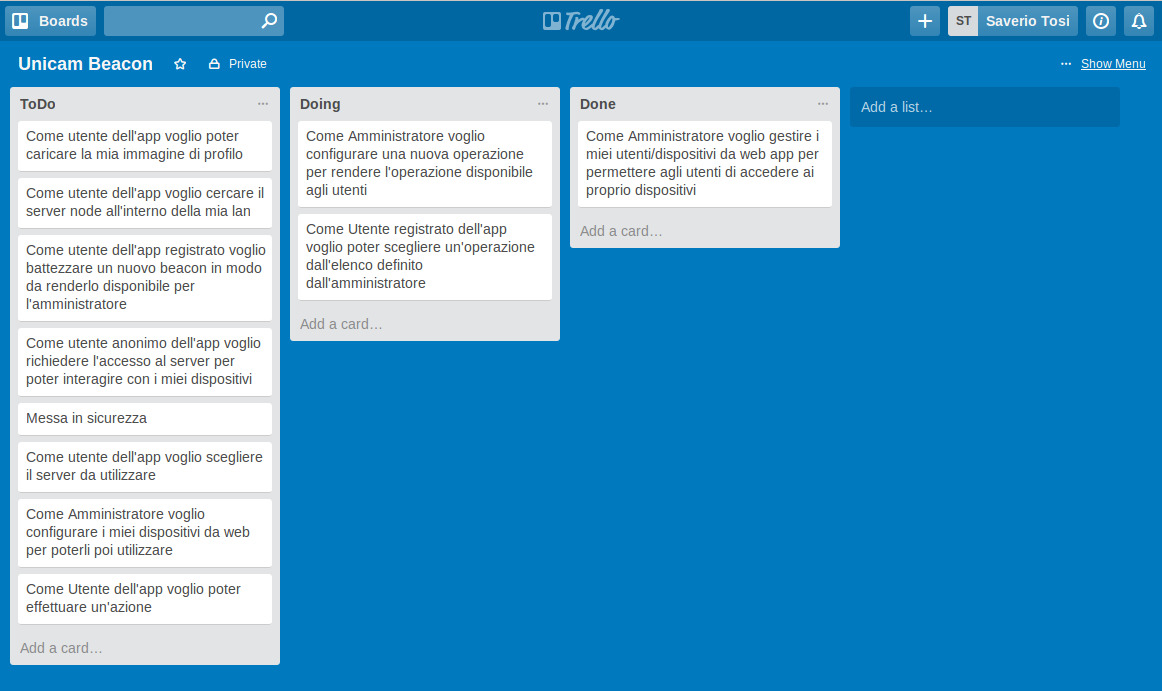
\includegraphics[scale=0.35]{Immagini/trello.png} 
\caption{Il nostro Trello, nella fase iniziale del progetto}
\end{figure}

\subsection{Analisi dei requisiti}
Si vuole realizzare un sistema per la domotica per d'ufficio, che oltre ad essere comandato con un'app, utilizzi i beacon per eseguire dei comandi automatizzati.

Il backend deve essere caricato su un RaspberryPI 2 e deve fornire i servizi REST sia per la webapp che per l'app mobile. 
Il backend, oltre a fornire le API REST\index{REST}, dove essere in grado di comunicare con il mondo esterno: sia con input che con degli output.
Per il prototipo, gli input saranno simulati con l'utilizzo di bottoni, nel prodotto finito essi saranno sostituiti con degli interruttori e dei sensori.
Gli output devono pilotare dei relè monostabili che permetteranno di comandare l'accensione/spegnimenti di luci, l'apertura di porte e di cancelli.

Il pannello di amministrazione è rappresentato dalla webapp a cui potrà accedere soltanto l'admin. 
Essa permette all'admin di gestire gli utenti dell'app dandogli e togliendogli privilegi, creare nuovi dispositivi da associare ai vari GPIO del RaspberryPI e   di configurare il modo in cui gli utenti possono interagire con i dispositivi: in maniera manuale, automatica(tramite beacon) o se per poter controllare il dispositivo è necessario trovarsi nelle vicinanze di esso. 

L'ultima componente è l'app mobile. 
Chi scaricherà l'app dovrà per prima cosa impostare l'indirizzo del server, se non si conosce l'indirizzo deve essere possibile fare una scansione della rete locale per trovare i backend attivi nella propria LAN. 
Una volta che si è connessi al server si può proseguire con il login/registrazione. La registrazione non abilita l'utente all'utilizzo di Proximity System, l'utente non potrà far nulla finché l'admin non gli dà i permessi per utilizzare l'app. 
Con l'app un utente ha due funzionalità: la prima è poter cercare nuovi beacon da segnalare all'amministratore; la seconda è interagire con i propri dispositivi.

{\Huge NOTA *** AGGIUNGERE DIAGRAMMA UML PER UTILIZZO APP ***}

\section{Miglioramento dell'esperienza utente}
Dopo una prima stesura del codice e la realizzazione di un primo prototipo,
abbiamo deciso migliorare l'esperienza utente dando la possibilità al server di inviare notifiche push ai client.
Per fare ciò, abbiamo utilizzato le WebSocket, una delle funzionalità più interessanti introdotta con l'HTML5.

Nel Capitolo \ref{chap:websocket} illustreremo come sia possibile migliorare le  prestazione di una generica WebApp che fornisce dei dati in tempo reale, per poi dimostrare come sia semplice utilizzare tale specifica, sopratutto se si utilizzano delle libreria ad hoc come Socket.io. 